% This is LLNCS.DEM the demonstration file of
% the LaTeX macro package from Springer-Verlag
% for Lecture Notes in Computer Science,
% version 2.4 for LaTeX2e as of 16. April 2010
%
\documentclass{llncs}
%
\usepackage{fixltx2e}
\usepackage{makeidx}  % allows for indexgeneration
%\usepackage{algorithm}
%\usepackage{algpseudocode}
\usepackage[ruled,vlined]{algorithm2e}
\usepackage{multirow}
\usepackage{amsmath}
\usepackage{xcolor}
\usepackage{wrapfig}
\usepackage{graphicx}

\renewcommand{\algorithmicrequire}{\textbf{Input:}}  % Use Input in the format of Algorithm
\renewcommand{\algorithmicensure}{\textbf{Output:}} % Use Output in the format of Algorithm

%
\begin{document}
%
\frontmatter          % for the preliminaries
%
\pagestyle{headings}  % switches on printing of running heads
%\addtocmark{Hamiltonian Mechanics} % additional mark in the TOC
%
%\chapter*{Preface}
%

%\vspace{1cm}
%\begin{flushright}\noindent
%\end{flushright}
%
%\chapter*{Organization}
%
%\section*{Executive Commitee}
%\begin{tabular}{@{}p{5cm}@{}p{7.2cm}@{}}
%\end{tabular}
%
%\section*{Program Commitee}
%\begin{tabular}{@{}p{5cm}@{}p{7.2cm}@{}}
%\end{tabular}
%
%\begin{multicols}{3}[\section*{Referees}]
%\end{multicols}
%
%\section*{Sponsoring Institutions}
%
%
%\tableofcontents
%
\mainmatter              % start of the contributions
%
\title{H}
%
\titlerunning{}  % abbreviated title (for running head)
%                                     also used for the TOC unless
%                                     \toctitle is used
%
\author{Zhimin Wu\inst{1} \and Yang Liu\inst{1}}
%
\authorrunning{Zhimin Wu et al.} % abbreviated author list (for running head)
%
%%%% list of authors for the TOC (use if author list has to be modified)
\tocauthor{}
%
\institute{NTU, NTU, SG,\\
\email{zwu010@e.ntu.edu.sg},\\ WWW home page:
\texttt{http://users/\homedir iekeland/web/welcome.html}
\and
Universit\'{e} de Paris-Sud,
Laboratoire d'Analyse Num\'{e}rique, B\^{a}timent 425,\\
F-91405 Orsay Cedex, France}

\maketitle              % typeset the title of the contribution

\begin{abstract}
The zhimin \dots
\keywords{cs}
\end{abstract}
%
\section{Introduction}
%
%
\section{Counterexample Generation in LTL Model Checking}
%
%
\section{GPU Architecture and CUDA Dynamic Parallelism}\label{sec:sec3}
%
%
\section{CUDA Counterexample Generation}
%

In this chapter, we will describe our CUDA Counterexample Generation proposal. The target of our design is to accelerate the Path Generation procedure in Counterexample generation by parallel the procedure in GPU, which is a parallel BFS-Related work. The important properties of BFS is that the node number in each level is changing. So in parallel BFS program, the tasks size is not consistent, which makes the task queue management and the load balance during the search important. These are all being taken into consideration in our design. Our design is based on the CUDA Dynamic Parallelism and Kepler GK110 Architecture, as well as the programming model. Firstly, we propose the overall design of CUDA Counterexample Generation Algorithm. Then we explain in detail about the Two-Level Queue Management and Two-level Task Schedule in our design. Finally we propose the Path Record during the Path Generation.

%
\subsection{CUDA Dynamic Path Generation Algorithm}
%

The original Counterexample Generation algorithm is shown in \ref{}. Our design is to build the general Path Generation Algorithm to accelerate the \textsl{Path} and \textsl{FindshortestPathtoSCC\&Acc} in the original algorithm. The overall scheme can be shown in \ref{fig:Overall}.

\begin{figure}[htbp]
	%\vspace{2.5cm}
	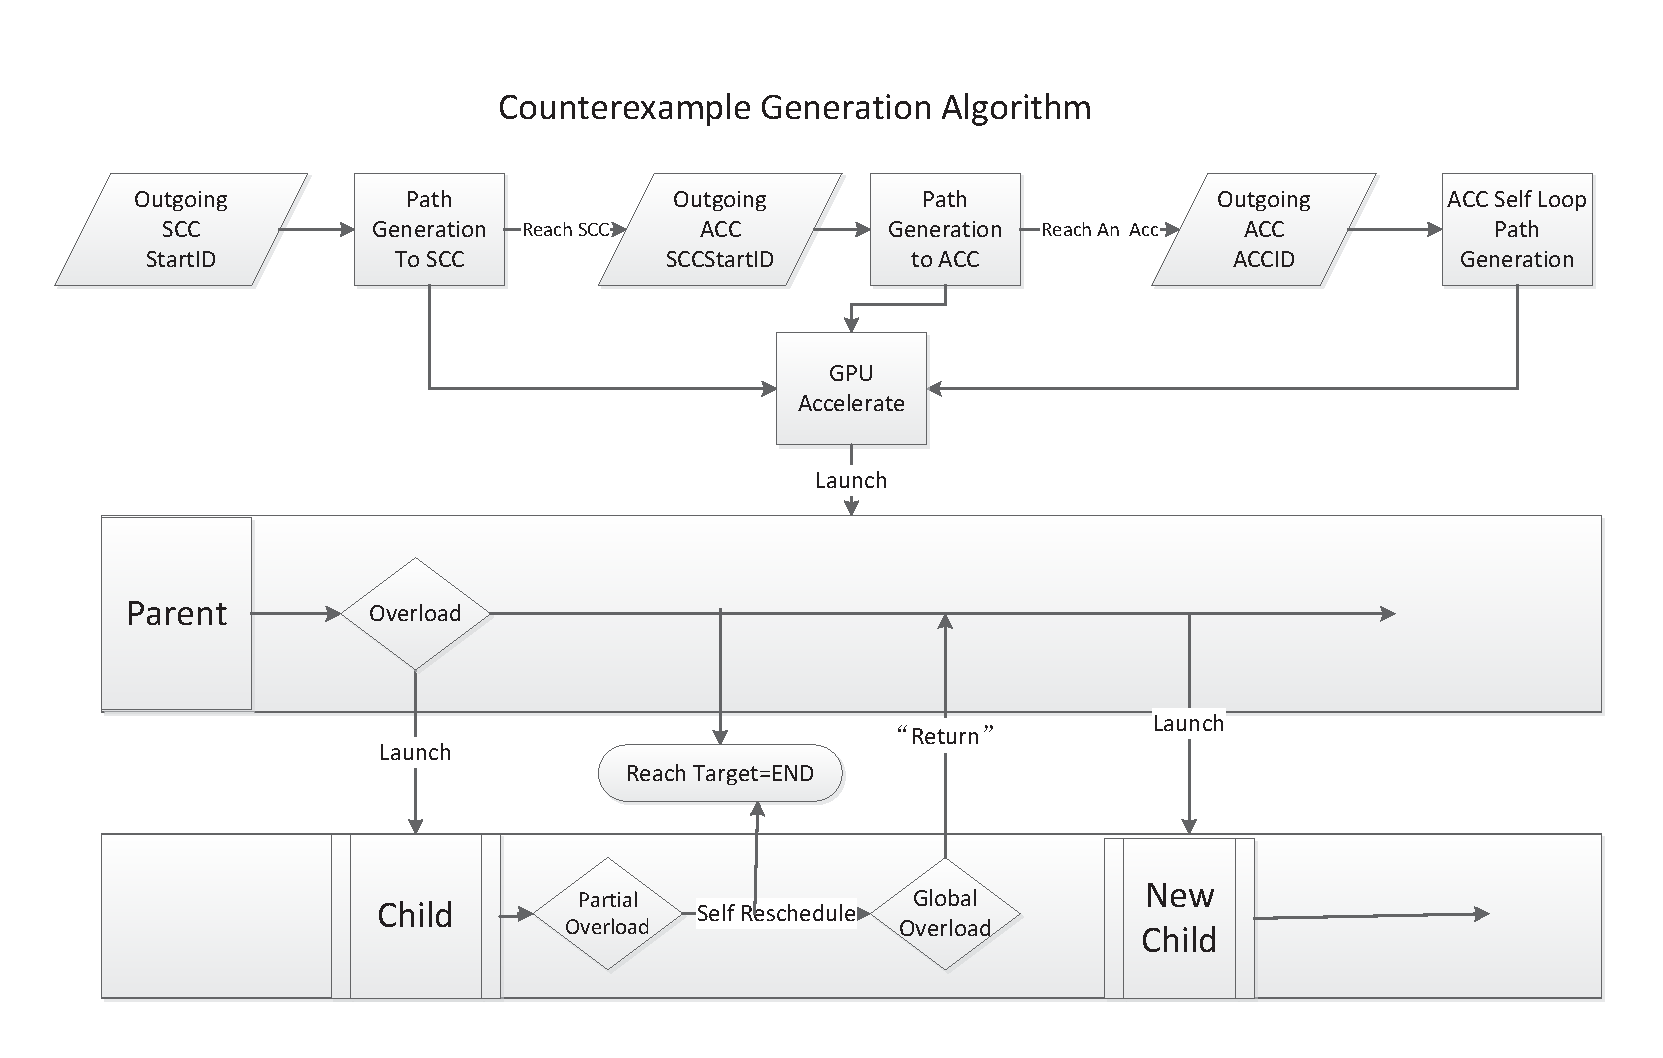
\includegraphics[width=\textwidth]{Overall.eps}
    \caption{Overall Design}
    \label{fig:Overall}
\end{figure}
	
In normal CUDA program, host will call the kernel to run in GPU with static grid and block structure. And in the previous research CUDA IIIT-BFS \cite{}, it need to launch the kernel each time when a level of the graph is explored, which is costly and slower than CPU-BFS. To deal with this problem, research CUDA UIUC-BFS \cite{} propose a hierarchical memory management proposal. It build three level queue for BFS to avoid consequently launch kernel, which result in a certain speedup. But it is still a static method that can not adjust according to the task size; and there is no load balance plan in it. In addition, the above research does not focus on model checking.

There is also some research on BFS-Related CUDA accelerated model checking algorithms.(to be continued...)

To deal with these problems. Our solution to CUDA Counterexample Generation is to utilizes Dynamic Parallelism of CUDA and features of GPU GK110 architecture. Then we got a new CUDA Dynamic Path Generation Algorithm shown in\ref{}. Totally Speaking, the feature we focus on is he amount of tasks during the execution of BFS is dynamically changing. Our algorithm contains four parts:

\begin{itemize}
    \item We utilize the CUDA Dynamic Parallelism to dynamically fork Child threads to fit the changing of tasks. We build a dynamic Parent-Child relationship.
    \item We build a Three-Level Queue Management proposal to fit the dynamic parallelism and dynamic task expanding.The three-level is made up of two physical level and a virtual level.
    \item We build a Two-level Dynamic Task Schedule to fit the dynamic Parent-Child relationship control and load balance.
    \item We utilize the hierarchical Memory in GPU to do the Two-Level Path Recording and duplicate elimination to some extent.
\end{itemize}

We present the pseudo-code of our algorithm in Algorithm $1$, Algorithm $2$ and Algorithm $3$: Algorithm \ref{alg:PGpath} propose the \textsl{CudaParentPathGeneration} Algorithm. It is the kernel launched by host.It contains the initial steps of Path Generation and will finish a certain amount of BFS-related tasks. It major focus on the Parent-level task schedule, Queue Management, fork Child-threads and distributed tasks to them. It controls the Parent-Child Relationship during the execution. Line X to Line X is

            %algorithm1
			\begin{algorithm}[htbp]
			%\fontsize{9pt}{9pt}\selectfont
			\caption{CudaParentPathGeneration Algorithm}
			\label{alg:PGpath}
			\begin{algorithmic}[1]
            \Require $Start\_ID, SCCnodelist/ACCnodelist, OutgoingRelation$
            \State $Define \_shared\_ S\_queue, Queuesize, Ifexpanded, IfSCC\/AccReach;$
            \If{$inblockthreadindex = 0$}
                \State $Three-levelQM: S\_queue.enqueue(Start\_ID);$
                \State $Path-Recording: path\_record\_queue inside StartNode;$
            \EndIf
            \State $Intra\_block_syn();$
            \While{$Ifexpanded \neq TRUE$}
                \If{$inblockthreadindex < Queuesize$}
                    \State $Three-levelQM:S\_queue.ParallelDequeue()$;
		            \State $CudaScc\&AccReach: SCC\&AccReach detection$;
		            \State $BFS, OutgoingRelation \Rightarrow NEXT level$;
		            \State $Path\-Recording:Inherit\&Update(path\_record\_queue of each Node);$
		            \State $Three\-levelQM:S\_queue.ParallelEnqueue();$
                \EndIf
                \If {$inblockthreadindex = 0$}
                    \State $Queuesize \Leftarrow S_queue.size;$
		            \If{$Queuesize > THRESHOLD$}
			             \State $Ifexpanded := TRUE;$
                    \EndIf
                \EndIf
            \EndWhile
            \State $Intra\_block_syn();$
            \If{$inblockthreadindex = 0$}
                \State $Prepare for parallelism expanding:$
                \State $Path Recording:copy back to Global memory$
		        \State $Two-levelTS: Parent-level Initial Task Schedule;$
		        \State $Three-LevelQM: Build \_device\_ G_queue;$
                \State $Update(Expanding\_ChildSize), Initial(\_device\_ G\_IfSCC\&AccReach);$
            \EndIf
            \State $Intra\_block_syn();$
            \While{$!IfSCC\&AccReach AND !G_IfSCC\&AccReach$}
	            \If{$inblockthreadindex = 0$}
		              \State $Three-levelQM: Build(\_device\_ V\_G\_Queue);$
	                  \State $Two-levelTS: ParellelCal(Child\_Tasks\_Offset\_V\_G\_Queue);$
                \EndIf
	            \If{$inblockthreadindex = 0$}
		              \State $ChildKernel<<<...>>>(V\_G\_Queue,Child\_Tasks\_Offset,...);$
                      \State $CudaDeviceSyn():If Childs NOT fit tasks OR finished, return to Parent;$
                      \State $Then Continue loop:Two-levelTS:Parent Reschedule tasks, Child re-expanding;$
                \EndIf
	        \EndWhile
            \State $Intra\_block\_syn()$;
            \end{algorithmic}
			\end{algorithm}

Algorithm \ref{alg:CGpath} propose the \textsl{CudaChildPathGeneration} Algorithm. It is the kernel launched by parent thread, regarded as Child kernel. It will finish the major tasks of Path Generation. It contains the Child-level Queue Management, Child-level task schedule and maintain the Parent-Child Relationship during the execution. Line X

            %algorithm2
            \begin{algorithm}[htbp]
            \caption{CudaChildPathGeneration Algorithm}
            \label{alg:CGpath}
            \begin{algorithmic}[1]
            \Require
            $\_device\_ V\_G\_Queue, Child\_Tasks\_offset, $ \\
            $SCCnodelist\/AccNodelist, OutgoingRelation$ \\
            $Pre-define \_device\_ (Child\_Expandedtask, Child\_syn\_need,$\\
            $Child\_need\_back2parent,G\_IfSCC\&AccReach)$
            \State $Define \_shared\_ (Child\_S\_Queue, queuesize, IfSCC\&Accreach);$
            \State $Get inblockthreadindex, globalthreadindex;$
            \If{$inblockthreadindex = 0$}
                \State $Initialize(queensize, IfSCC\&Accreach);$
            \EndIf
            \If{$globalthreadindex = 0$}
                \State $Initialzie(all \_device\_ variables);$
            \EndIf
            \State $CudaInterBlockSyn();$
            \While{$!G_IfSCC\&AccReach AND !Child\_need\_back2parent$}
	            \State $BlockTasks := Tasksoffsets[blockindex + 1] - Taskoffsets[blockindex];$
	            \State $Three-levelQM: Enqueue(Getthreadtask FROM V\_G\_Queue);$
                \State $Queuesize \Leftarrow blocktasks.num;$
                \State $Intra\_block\_syn();$
	            \If{$inblockthreadindex < queuesize$}
		             \State $Three-levelQM:Child\_S_Queue.ParallelDequeue();$
		             \State $CudaScc\&AccReach: SCC\&AccReach detection;$
                            \If{$Reach SCC$}
                                \State $G\_IfSCC\&AccReach := TRUE, Record Path;$
                                \State $BREAK;$
                            \EndIf
		             \State $BFS{}, OutgoingRelation \Rightarrow NEXT level;$
		             \State $Path-Recording:Inherit\&Update(path\_record\_queue of each Node);$
                     \State $IFDuplicate \Leftarrow Path-Recording();$
                            \If{$IFDuplicate = TRUE$}
                                \State $CONTINUE;$
		             \State $Three-levelQM:S\_queue.ParallelEnqueue();$
	            \EndIf
                \State $Intra\_block\_syn();$
	            \If{$inblockthreadindex = 0$}
		             \State $queuesize \Leftarrow Child\_S\_Queue.size;$
		             \If{$queuesize > block Threshold)$}
			             \State $Child\_syn\_neede := TRUE;$
                     \EndIf
                \EndIf
	            \State $CudaInterBlocksSyn();$
	            \If{$child\_syn\_needed = TRUE$}
		            \State $Three-levelQM: Parallel\_Update(G\_Queue)$;
                    \If{$globalthreadindex = 0$}
                        \State $Build(V\_G\_Queue);$
                        \State $Two-levelTS: Inter\_Childblocks\_Tasks\_Reschedule;$
            		    \If{$Whole\_blocks\_overloaded = TRUE$}
			                 \State $Child\_return2Parent := TRUE;$
                        \EndIf
			         \EndIf
                     \State $CudaInterblocksSyn();$
                \EndIf	
            \EndWhile
            \State $CudaInterblocksSyn();$
            \end{algorithmic}
            \end{algorithm}

Algorithm \ref{alg:Algmulti} propose the \textsl{CudaQuicksort},\textsl{Scc\&AccReach} and \textsl{CudaBlocksSyn} Algorithm. \textsl{CudaQuicksort} algorithm utilize the Dynamic Parallelism feature of CUDA to do quick sort for SCC node list.This refer to \ref{}. \textsl{Scc\&AccReach} use the Binary search to find if the path generation execution has reached SCC. \textsl{CudaInterBlocksSyn} Algorithm refers to the algorithm mentioned in \ref{}. It choose the \textsl{simple\_blocks\_synchronize} when the number of blocks is small. And the \textsl{tree\_blocks\_synchronize} is for large number of blocks.

            %algorithm 3
            \begin{algorithm}[htbp]
            \caption{CudaQuicksort, Scc\&AccReach and CudaInterBlocksSyn Algorithm}
            \label{alg:Algmulti}
            \begin{algorithmic}[1]
            \State $CudaQuickSort(data, pivot, left, right)$
                \State $Define nleft,nright;$
                \State $Partition(data+left, data+right, pivot, nleft, nright);$
                \If{$left < nright$}
                    $CreatCudastream(s1);$
                    $CudaQuickSort<<<...s1>>>(data, left, nright);$
                \EndIf
                \If{$nleft < right$}
                    $CreateCudasteam(s2);$
                    $CudaQuickSort<<<...s2>>>(data, nleft, right);$
                \EndIf
                \\
            \State $Scc\&AccReach()$
                \State $Normal Binary Search$
                \\
            \State $CudaInterBlocksSyn()$
                \If{$blocks.num < THRESHOLD$}
                    $simple\_blocks\_synchronize();$
                \Else
                    $tree\_blocks\_synchronize();$
                \EndIf
            \end{algorithmic}
            \end{algorithm}

From the overall introduction of algorithms, the structure of our solution to the CUDA counterexample generation is clearly. Totally speaking, we utilize the dynamic parallelism technique from latest CUDA. But the key point is that we finish a complete scheme to make our algorithm available to utilize this support from cuda, as well as fit the new GK110 architecture. Then we reach the ultimate goal of working out a novel CUDA counterexample generation scheme. In the following parts, more detail will be introduced.

%
\subsection{Dynamic Parent-Child Relationship}
%

Data-dependent parallel work can be generated inline with CUDA Dynamic Parallelism\ref{}. So building the relationship between \textsl{Parent} and \textsl{Child} is a data-driven work. In our algorithm design, in order to maximize the utilization of parallelization, each thread is asked to just do the breadth search and path recording of one node. It means the number of nodes in each level of BFS will decide the needed threads number. Therefore, with the node number uncertainty in BFS-related Path Generation, the best way is to allocate threads during runtime. That is what our algorithms do. And in order to save the cost, our \textsl{Parent}, which is launched by host, should not be a large scale grid. The major tasks of path generation should be done by \textsl{Child} and the \textsl{Parent} focus on the initial steps of path generation and the \textsl{Parent-Child} relation management. In our algorithm, \textsl{Parent} will always be just one \textsl{block}. As the minimum source schedule unit in GPU is \textsl{warp}, the GK110 can support \textsl{$4$ warps} running at the same time, we always choose $4-warps\times\alpha$ as the threads number of \textsl{Parent} grid.

We show the relationship in \ref{fig:PCRelation}, The \textsl{Parent-Child} relationship is not static. when \textsl{Parent} launch \textsl{Child}, it will base on the current tasks to decide the structure of \textsl{Child}, the future tasks can not be forecasted but it is certainly that \textsl{Parent} should not set a very huge \textsl{Child} grid to prevent task overload. So in most case, \textsl{Parent-Child} relationship is dynamically adjusted. In our algorithm, when the total tasks overload in \textsl{Child},it should return to \textsl{Parent} for reallocating(shown in \ref()). However, launch \textsl{Child} for a lot of time is also costly. so we should make a compromise.It will be mentioned in the Dynamic Two-level Task Schedule part.

\begin{figure}[htbp]
    %\vspace{2.5cm}
    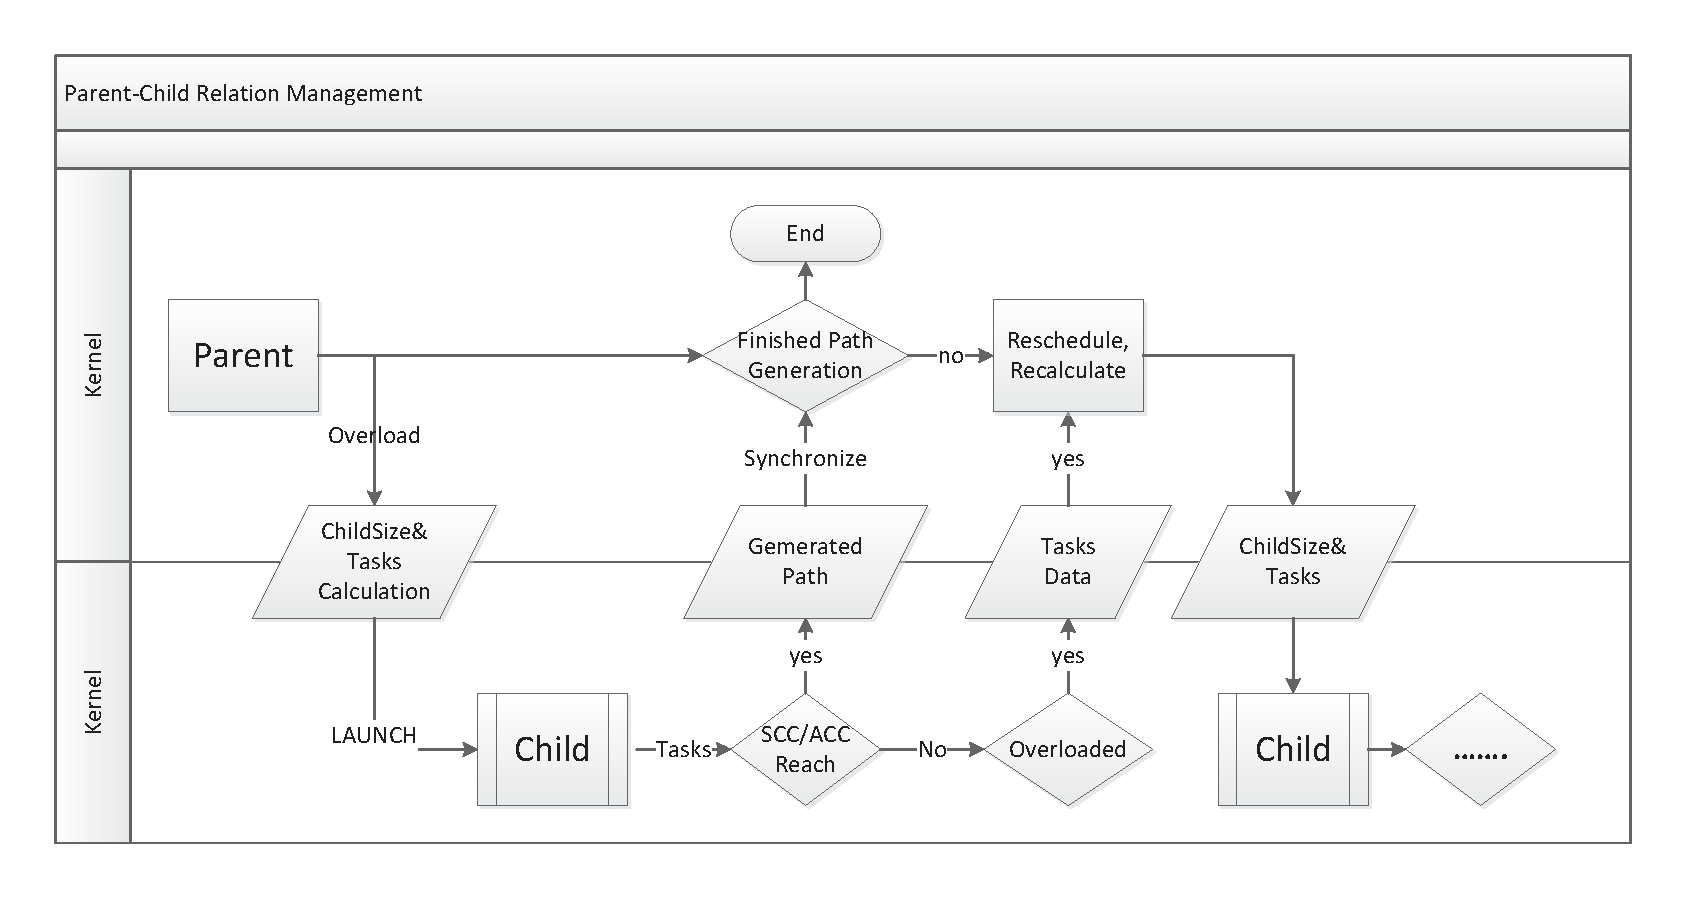
\includegraphics[width=\textwidth]{PCRelation.eps}
    \caption{Parent-Child Relationship}
    \label{fig:PCRelation}
\end{figure}

Beside the total tasks overload in \textsl{Child}, when the \textsl{generated path} in any thread in \textsl{Child} reach the SCC\/ACC ($SCCnodelist\\Accnodelist \cup Nodelist_in_path \neq \emptyset$), all threads in \textsl{Child} should synchronize and send result to \textsl{Parent}. As we mentioned in section XXX, The only way of communication between \textsl{Parent} and \textsl{Child}, as well as among \textsl{Childblocks} is on \textsl{Global Memory}, so the thread that find SCC-reach will record the generated path and a mark in \textsl{Global Memory} then synchronise among all Child blocks. As a result, \textsl{Parent} will got the mark and result and exit the execution.

In total, The \textsl{Parent-Child} relationship is dynamic according to the task overload and SCC Reach. This is very flexible and can fully utilize the dynamic parallelism.It makes our CUDA Path Generation a on-the-fly algorithm.
%
\subsection{Dynamic Three-level Queue Management}
%

As we mentioned in \ref{sec:sec3}, the architecture of Memory in GPU contains Global memory and Shared Memory. Global memory can be read\/write by all blocks running in all SM and Shared Memory is just available to blocks in same SM. Read\/Write operation in Shared Memory cost much less than operation in Global Memory. We should utilize this feature to improve the performance of our algorithm. But the size of shared memory is much lower than Global Memory. For our algorithm that refer to huge data size, we can not get rid of visiting Global memory. Considering the point in dynamic parallelism that only when tasks overload then call Child, we build a dynamic hierarchical Queue to utilize the hierarchical memory. In order to fit our dynamic parallelism design, we build a Three-Level Queue Management scheme. The structure can be shown in \ref{fig:DQM}

\begin{figure}[htbp]
    %\vspace{2.5cm}
    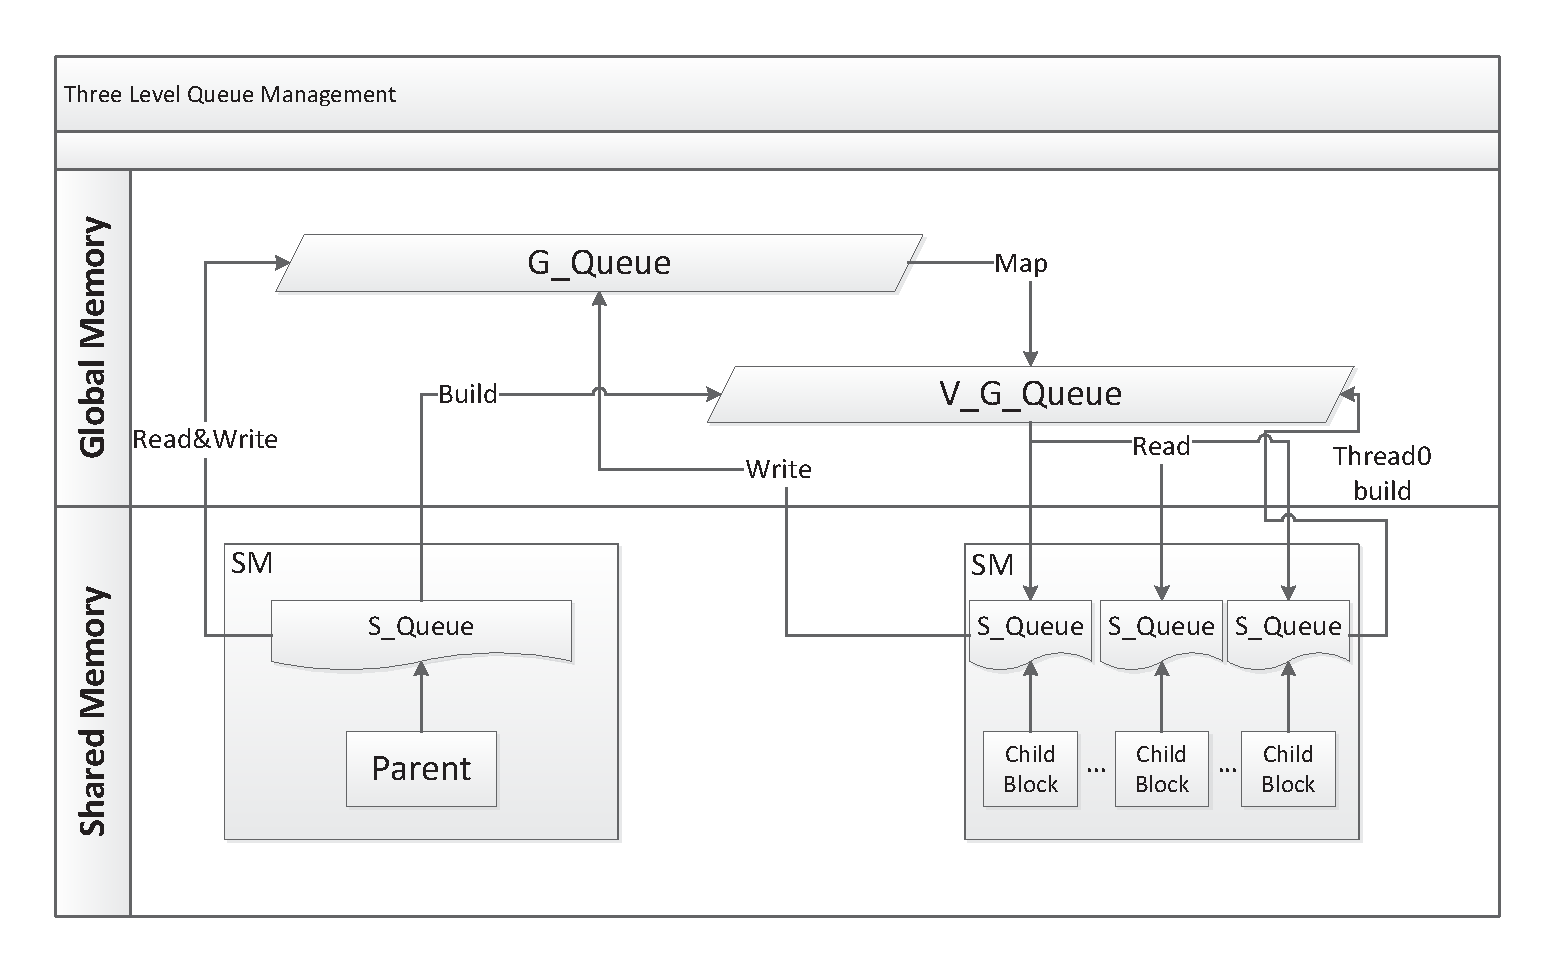
\includegraphics[width=\textwidth]{DQM.eps}
    \caption{Dynamic Three-level Queue Structure}
    \label{fig:DQM}
\end{figure}

The first level queue is stored in Shared Memory, marked as \textsl{S\_Queue}, It is shared among blocks in 1 SM. The second level queue is stored in Global Memory, marked as \textsl{G\_Queue}. The third level queue is also stored in Global Memory, called Virtual Global Queue, marked as \textsl{V\_G\_Queue}.

\textsl{S\_Queue} is the first task storage queue. When the BFS-related path generation begin, the expanded node ID will firstly be pushed into the \textsl{S\_Queue} in corresponding SM. Then for the next level expanding, threads do not need to visit Global Memory, it improve the data access speed. Here, the problem is it may cause read\/write conflict when parallel threads write/read at the same time. Then if we set lock or use atomic operation to prevent conflict, it will cost much with frequently write request at the same time. So based on the GPU SM architecture and new Warp schedule in $Kepler GK110$,we build the lock-free \textsl{S\_Queue} in structure showed in \ref{fig:SQueue}. As mentioned, the kernel is actually executed in groups of $32$ threads,called a \textsl{warp}. In $Kepler GK110$, it can support $4$ \textsl{warps} executing at the same time in reality. So for each block, we make the \textsl{S\_Queue} a four queue-group with $32$ queues each. So even the threads executed in a SM is much more than 4 \textsl{warps}, the number to write into queue at the same time is limited. \textsl{S\_Queue} is the queue directly accessed by threads during execution. As one thread only hold 1 task in each level search, if the tasks in \textsl{S\_Queue} exceed the number of threads executed in one block, the tasks should be re-scheduled and then it need to be transferred to \textsl{G\_Queue} in Global Memory.

\begin{figure}[htbp]
    %\vspace{2.5cm}
    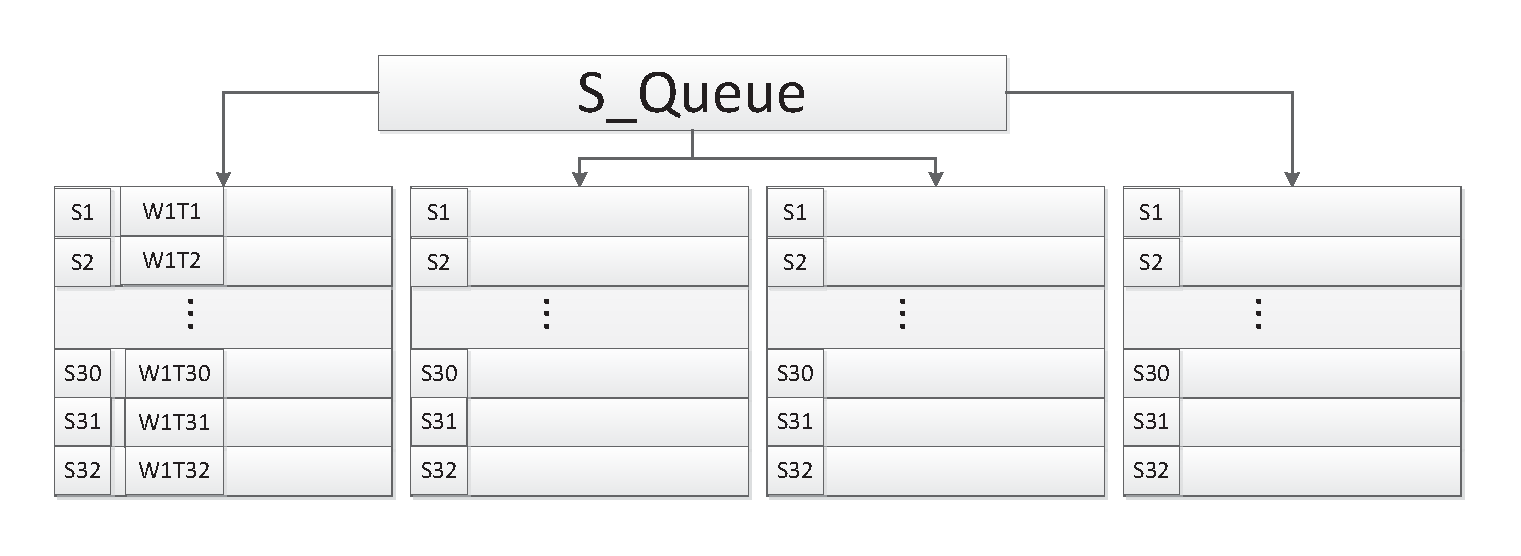
\includegraphics[width=\textwidth]{SQueue.eps}
    \caption{Structure of S\_Queue}
    \label{fig:SQueue}
\end{figure}

\textsl{G\_Queue} is build at the first time \textsl{Parent} call \textsl{Child}, it is a group of array. As dynamic allocate memeory and visit global memory is costly, this queue won't change after being build. As Global Memory is the way \textsl{Parent} communicate with \textsl{Child},it work as the way to transfer tasks to \textsl{Child} when the first time launching \textsl{Child}. Then in following execution, it stores the tasks when blocks overload and copy the content in \textsl{S\_Queue} to it. It is only visible for writing and \textsl{Child} threads will never directly read from it. The way to write \textsl{G\_Queue} is shown in \ref{fig:GQueue}.

\begin{figure}[htbp]
	%\vspace{2.5cm}
    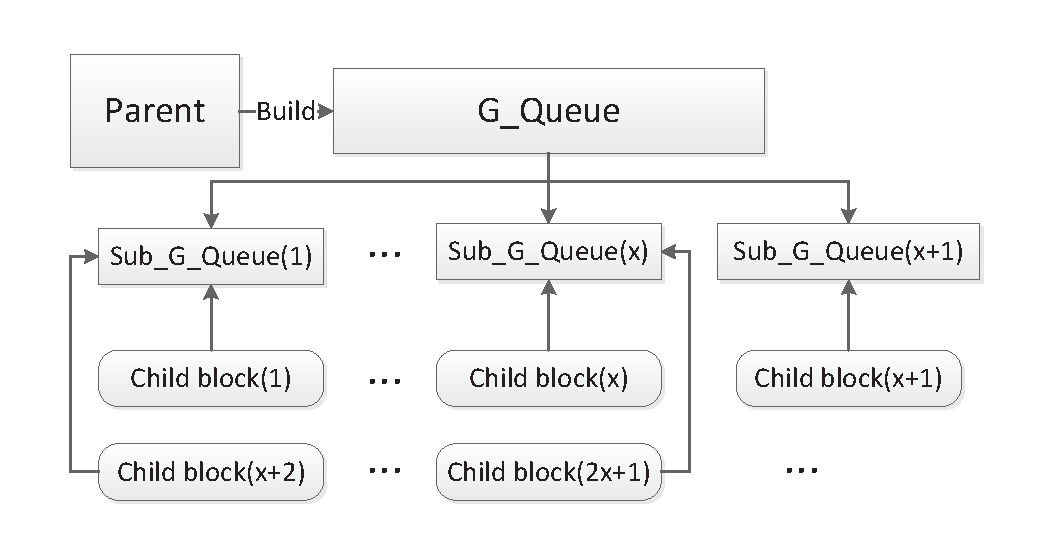
\includegraphics[width=\textwidth]{GQueue.eps}
	\caption{Structure of G\_Queue}
	\label{fig:GQueue}
\end{figure}

The Virtual Global Queue is the third level and it is a pointer array. As shown in \ref{flg:VGQueue}, in global view, the tasks store in the \textsl{G\_Queue} is not continuous. So it is not convenient for tasks reschedule as it will request a lot of computing on the task range for each thread. Then \textsl{V\_G\_Queue} is to build a continuous list for task schedule. It is only visible for reading by threads. And only \textsl{V\_G\_Queue} is dynamic built during execution. It can be shown in \ref{fig:VGQueue}.

\begin{figure}[htbp]
	%\vspace{2.5cm}
    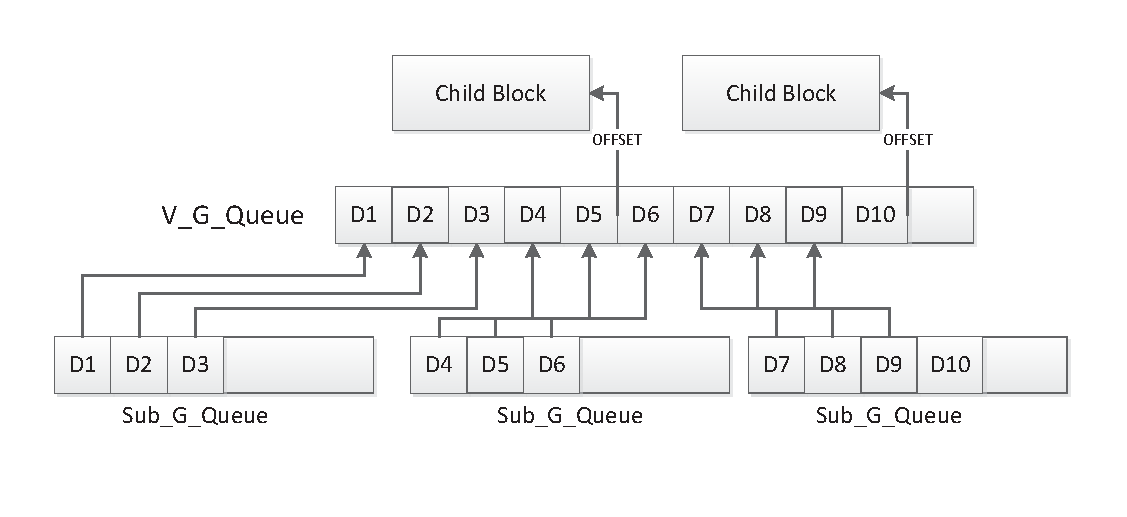
\includegraphics[width=\textwidth]{VGQueue.eps}
	\caption{Structure of V\_G\_Queue}
	\label{fig:VGQueue}
\end{figure}

This three-level Queue follows the rules of dynamic parallelism, aiming at building a flexible way of data access and improving the performance. It can work well with the \textsl{Parent-Child} structure.
%
\subsection{Dynamic Two-level Task Schedule}
%

In previous sections, what we mentioned contains two conditions that program need to do task reschedule:
   \begin{itemize}
        \item when \textsl{Parent} finish some initial steps of BFS-related path generation and can not hold more tasks, it need to call \textsl{Child} and schedule tasks to \textsl{Child} the first time.
        \item when the whole tasks make \textsl{Child} blocks overloaded, it need to return to \textsl{Parent} to rearrange the \{Child} grid so as to reschedule the tasks
   \end{itemize}

In this two conditions, tasks schedule is done by \textsl{Parent}. And launching kernel is an expensive work. If just one or a few blocks in \textsl{Child} is overloaded, it is obviously that the execution should not return to \textsl{Parent}. Instead, inside the \textsl{Child}, it should also have a \textsl{Child level inter blocks} task schedule. That, combined with the \textsl{Parent} level task schedule, we build the two-level task schedule. It can be shown in \ref{fig:TwoTS}.

\begin{figure}[htbp]
    %\vspace{2.5cm}
    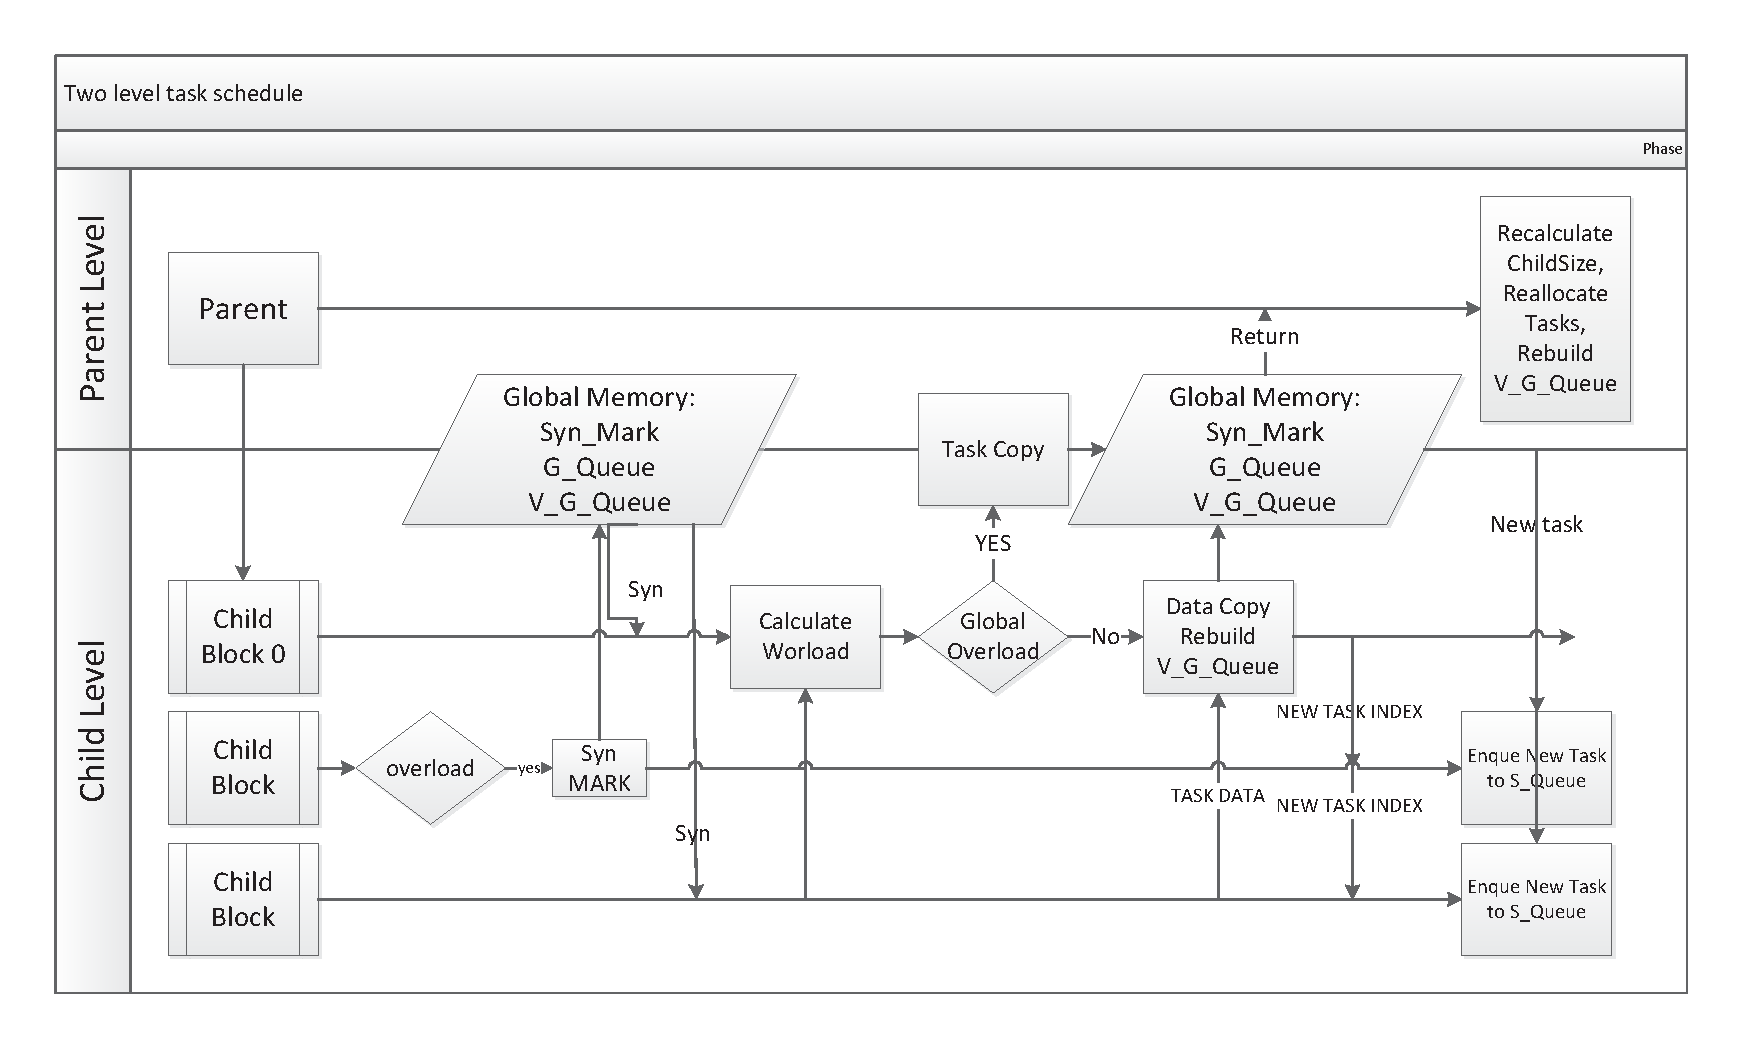
\includegraphics[width=\textwidth]{TwoTS.eps}
    \caption{Dynamic Two-level Task Schedule}
    \label{fig:TwoTS}
\end{figure}

In \textsl{Child} blocks, after each level of path generation, each block will decide if overloaded. Then if so, block will copy tasks in its own \textsl{S\_Queue} back to \textsl{G\_Queue}. Then mark \textsl{Child\_syn\_needed} in order to make all other blocks enter the \textsl{Child level} tasks schedule. In our algorithm, the \textsl{Child level} tasks schedule will balance the tasks among all blocks by build new \textsl{V\_G\_Queue}. This behavior has no reference to \textsl{Parent}. Here, in order to make each block has enough resource to do future expanding, the schedule should not make the new tasks in each block exceed a \textsl{threshold}, Or the algorithm will conclude that the \textsl{Child} is overloaded.

Then it will come to \textsl{Parent level} task schedule. \textsl{Parent} will calculate new \textsl{Childsize-Child blocks number}, build new \textsl{V\_G\_Queue} and calculate tasks offset for each \textsl{Child block}. Here it also comes to the problem that if \textsl{Childsize} is not appropriate, then the \textsl{Child} will return to \textsl{Parent} frequently, which is costly. To make a compromise, in operation line X in our algorithm, when calculating the \textsl{Childsize}, we guarantee that tasks allocated to each Child should not beyond the number $\textsl{warpsize = 32}$ and the threads number in each \textsl{Child block} should be $warpsize\times\alpha$.

%
\subsection{Two-level Path Recording and Duplicate Elimination}
%

Our algorithm is to deal with the Path Generation so as to get Counterexample. So path recording is necessary. Since the path generation is a BFS-related work, the path record is updated in each search level. Take \ref{fig:PathRExp} as an example, the nodes in each level will inherit their precusor's path and then add themselves in the path. When a node has more than one precursor, it will inherit more than one path. However, our algorithm is to find a path to reach $SCC\/ACCnodelist$, only to inherit one path is enough and this will save the storage space. Then we build the Path Recording scheme according to this and also the dynamic parallelism feature inclued in all other parts.

\begin{figure}[htbp]
	%\vspace{2.5cm}
    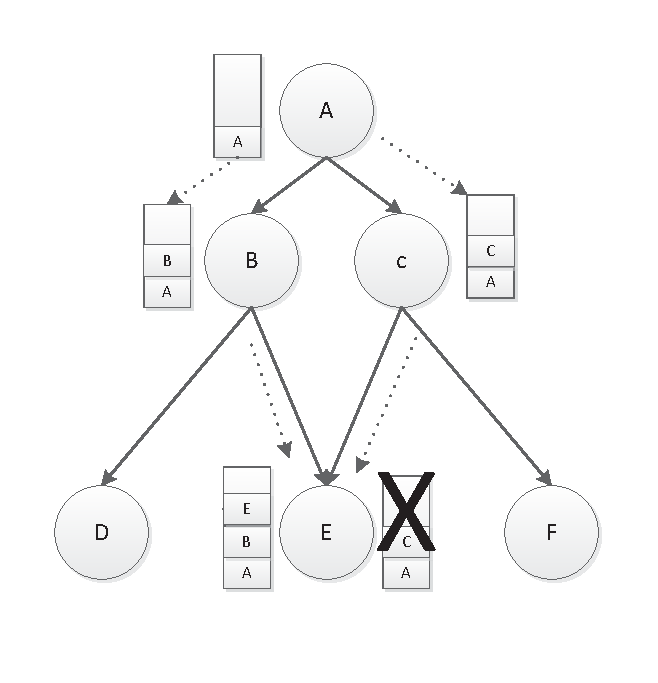
\includegraphics[width=\textwidth]{PathRExp.eps}
	\caption{Path Recording Example}
	\label{fig:PathRExp}
\end{figure}

We call our scheme \textsl{Two-level Path Recording}. One is Shared Memory level path recording and the other is Global Memory level. Firstly, a simple structure is defined:

\begin{center} $PathRecordNode{nodeid, pathqueue}$\end{center}

Then we define a \textsl{PathRecordNodeList} array in each block that stored in Shared Memory (called \textsl{S\_PRN\_List}) and one more array in Global Memory (called \textsl{G\_PRN\_List}. On a whole, during the path generation, threads will update the path in corresponding node in Shared Memory following the inherit rules mentioned. And the updating of path in Global Memory happens when the overload happens in order to fit the dynamic tasks schedule design previously mentioned. In details, the steps to do the path recording are as follows, all these steps are executed after the \textsl{IfReachSCC\&ACC} detection of current visiting node:

\begin{itemize}
	\item when a node is being visited, update the corresponding \textsl{PathRecordNode} in the \textsl{S\_PRN\_List} by push itself to the path
	\item when a node is being visited, copy its updated path to each of its successor's corresponding path queue If it is empty. If not, it means the successor has inherit a path and there is no need to inherit another path. Here, it also means the successor has been put into task queue and it can eliminate the duplication inside a block to some extent
	\item when overload happen, we do the path copy together with copy tasks from \textsl{S\_Queue} to \textsl{G\_Queue}. Only the path data that with ID contained in \textsl{S\_Queue} are copied. Here, with the same rule, if the corresponding \textsl{PathRecordNode} has unempty path queue, the copy operation will be aborted and this node ID will also be aborted in task copy.
	\item these steps continue until \textsl{IfReachSCC\&ACC} detection return TRUE.
\end{itemize}

Here, the reason we say it can just eliminate duplication to some extent is that after once \textsl{$S\_PRN\_List \Rightarrow G\_PRN\_List$} copy, All path queue in \textsl{$S\_PRN\_List$} will be empty. So in following steps, the visited node may have possibility to be visited again and it will store the path again. But when copy back to \textsl{G\_PRN\_Queue}, this will be detected.

Another problem is the storage space problem. (need expanding, to be continued...)

In addition, when a thread updating the path queue in \textsl{PathRecordNode}, atomic operation is needed to prevent conflict. And it should not block other threads. This will be discussed in the following part.
%
\subsection{Synchronization and Atomic Operation}
%
In our algorithm, synchronization contains two parts: intra block synchronization and inter block synchronization. For all threads inside a block, the intra block synchronization should be taken in each level expanding as the algorithm need to judge if overload happen. This intra block synchronization has been supported by CUDA with $CudaThreadSync()$. What we should focus is the inter block synchronization. It requires all blocks to attend, So a low-cost way to do this is necessary. We chose the inter block synchronization method in \cite{} that has been proved to be high efficiency. the data that \textsl{Child}  blocks need to communicate with each other contains \textsl{IfSCC\/AccReach, If overload and If\_return2Parent}. These are stored in Global Memory and will be checked by each thread in each level expanding. If the corresponding event happens being detected by any thread, it will utilize atomic operation to update the data in Global Memory and then called the \textsl{CudaInterBlocksSyn}. After other blocks detect the update, they will also call \textsl{CudaInterBlocksSyn} so as to synchronise among all blocks.

Here we mention the atomic operation. It is used to build a unblock lock. When some threads want to write the same memory address at the same time, only the first one call the lock will get the access right and the other will abort their write operation and continue their executing. The design of this lock is shown in \ref{alg:atomiclock}

\begin{algorithm}[htbp]
\caption{Unblock lock with atomic operation}
\label{alg:atomiclock}
\begin{algorithmic}[1]
\While{$Iffinished = TRUE$}
    \If{$Atomic(&mutex, 1)$}
        \State write operation;
        \State $Iffinished := True;$
        \State $Atomic(&mutex, 0);$
    \Else
        \State $abort = TRUE;$
        \State $break;$
    \EndIf
\EndWhile
\end{algorithmic}
\end{algorithm}

With all these above, we build the complete CUDA Path Generation algorithm for Counterexample Generation. All content make full use of the dynamic parallelism and the feature of new Kepler $GK110$ architecture.

%
\section{Implementation of Algorithm in PAT}
%

%
\section{Experiments and Evaluation}



%
% ---- Bibliography ----
%
\begin{thebibliography}{}
%


\end{thebibliography}
%\clearpage
%\addtocmark[2]{Author Index} % additional numbered TOC entry
%\renewcommand{\indexname}{Author Index}
%\printindex
%\clearpage
%\addtocmark[2]{Subject Index} % additional numbered TOC entry
%\markboth{Subject Index}{Subject Index}
%\renewcommand{\indexname}{Subject Index}
%\input{subjidx.ind}
\end{document}
